\documentclass[letterpaper, 10 pt, conference]{IEEEtran}
%\documentclass[a4paper, 10pt, conference]{ieeeconf}

\usepackage[T1]{fontenc}
\usepackage[utf8]{inputenc}

\usepackage{tikz}
\usetikzlibrary{calc,patterns,angles,quotes,shapes}
\usepackage{subcaption}

\usepackage{graphics}
\usepackage{mathptmx}
\usepackage{times}
\usepackage{amsmath}
\usepackage{amssymb}

\title{\LARGE \bf The TransHumUs project for the French Pavilion \\ at La Biennale di Venezia 2015}

\author{Guilhem Saurel, Michel Taix and Jean-Paul Laumond}

\begin{document}

\maketitle
\thispagestyle{empty}
\pagestyle{empty}

\begin{abstract}
    TODO
\end{abstract}

\section{When robotics meets art}
\subsection{The transHumUs project of Céleste Boursier-Mougenot}

\begin{figure}[thpb]
    \centering
    \includegraphics[width=\linewidth]{img/vue_artiste.jpg}
    \caption{Artist's Impression}
    \label{artists_impression}
\end{figure}

For the 56th edition of the Venice Biennale International Contemporary Art Exhibit, Céleste Boursier-Mougenot composed a poetic work evoking the follies of 18th-century romantic parks, while revealing its political dimension.

With rêvolutions by artist Céleste Boursier-Mougenot, accompanied by the exhibit’s Curator, Emma Lavigne, the French Pavilion of the Venice Biennale has been transformed into an organic, dreamlike isle.

Under the glass roof, with the Pavilion’s flight and tree-lined lanes of the Giardini, Céleste Boursier-Mougenot has rolled out the choreography of three mobile trees moving according to their metabolism, the varying flow of their sap and their sensitivity when going from shadow to light.

\subsection{The robotics interpretation}

TODO interpretation → discours sur le mouvement

\section{The robotic project}
\subsection{Specifications}

Acording to the artist's wishes, we established the initial specifications for the piece of art, in order to find the right industrial partners:

\begin{itemize}
    \item The artwork will be composed by three trees of approximately 4 to 5 meters high and 3 tons;
    \item They will move in accordance with some feedback from their metabolism;
    \item The movement will be holonomic in a plane;
    \item The trees will have to move silently;
    \item The motion must be really slow, hardly perceptible (between 0 and 1 meter per minute);
    \item The trajectory shall cover as much as possible the available space;
    \item Several trees will have to coordinate themselves in the same area;
    \item The wheelbase must be able to roll on soft floors (mud and gravels) as well as on hard ones (concrete).
\end{itemize}

\subsection{Technical solutions}

\paragraph{Sapflow sensors} have been selected by biology researchers as they can provide a reliable signal correlated with the tree's metabolism.

\paragraph{Automatic Guided Vehicles} (AGV) with three directable wheels should comply with the admissible mechanical load on the concrete and provide an overall holonomic motion possibility.

\paragraph{Absolute geolocation} that works well indoor and outdoor, including on bumpy areas, at an affordable price is hard to find, but exists.

\subsection{Architecture for the generation of motion}

As the artist wants an holonomic planar motion, in the most basic form, we need input 3 variables. The artist also wish that the trees behave in a similar manner in whatever direction it goes, so we choose a polar coordinate system concentric with the AGV: $(v, \theta, \omega)$, where:

\begin{itemize}
    \item $\theta \in [0, 2\pi[$ is the direction of the center of the AGV;
            \item $v \in [-1, 1]$ is its linear velocity along the direction $\theta$;
            \item $\omega \in [-1, 1]$ is its angular velocity.
        \end{itemize}

        With this system, we can easily compute the output needed by the AGV, which consist of the orientation $\theta_i$ of each wheel and its traction velocity $v_i$:

        \begin{eqnarray*}
            v_{xi} &=& v \cos(\theta)- \omega \sin(\alpha_i) \\
            v_{yi} &=& v \sin(\theta)+ \omega \cos(\alpha_i) \\
            v_i &=& \sqrt{v_{xi}^2 + v_{yi}^2} \\
            \theta_i &=& \arctan(v_{yi}, v_{xi})
        \end{eqnarray*}


        \begin{figure}[thpb]
            \centering

            \begin{subfigure}{.5\textwidth}
                \centering
                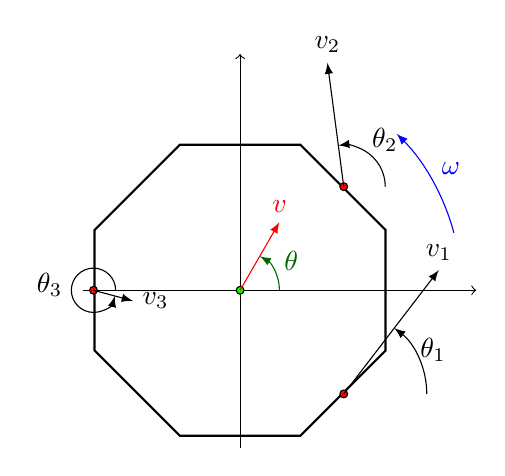
\begin{tikzpicture}
                    \draw [->] (-2, 0) -- (3, 0);
                    \draw [->] (0, -2) -- (0, 3);
                    \coordinate (o) at (0, 0);
                    \coordinate (v) at (0.5, {sqrt(3) / 2});
                    \coordinate (x) at ({+sqrt(2) / 2}, {sqrt(2) / 2});
                    \coordinate (y) at ({-sqrt(2) / 2}, {sqrt(2) / 2});
                    \coordinate (z) at (0, -1);
                    \draw (o) node [draw, thick, minimum size=4cm, name=O, regular polygon, regular polygon sides=8] {};
                    \draw (O) node [fill=green, circle, draw, inner sep=1pt] {};
                    \coordinate (a) at (O.side 6);
                    \coordinate (b) at (O.side 8);
                    \coordinate (c) at (O.side 3);
                    \coordinate (d) at (O.side 7);
                    \coordinate (e) at ($ (d) + (0, 0.5) $);
                    \coordinate (f) at ($ (a) + (1, 0) $);
                    \coordinate (g) at ($ (b) + (1, 0) $);
                    \coordinate (h) at ($ (c) + (1, 0) $);
                    \coordinate (i) at ($ (a) + (v) + (x) $);
                    \coordinate (j) at ($ (b) + (v) + (y) $);
                    \coordinate (k) at ($ (c) + (v) + (z) $);
                    \draw (a) node [fill=red, circle, draw, inner sep=1pt] {};
                    \draw (b) node [fill=red, circle, draw, inner sep=1pt] {};
                    \draw (c) node [fill=red, circle, draw, inner sep=1pt] {};
                    \draw [->, -latex, red] (o) -- (v) node [above] {$v$};
                    \pic [blue, draw, ->, -latex, "$\omega$", angle eccentricity=1.1, angle radius=80] {angle = e--o--b};
                    \draw [->, -latex] (a) -- (i) node [above] {$v_1$};
                    \draw [->, -latex] (b) -- (j) node [above] {$v_2$};
                    \draw [->, -latex] (c) -- (k) node [right] {$v_3$};

                    \pic [black!60!green, draw, ->, -latex, "$\theta$", angle eccentricity=1.5] {angle = d--o--v};
                    \pic [draw, ->, -latex, "$\theta_1$", angle radius=30, angle eccentricity=1.2] {angle = f--a--i};
                    \pic [draw, ->, -latex, "$\theta_2$", angle radius=15, angle eccentricity=1.5] {angle = g--b--j};
                    \pic [draw, ->, -latex, "$\theta_3$", angle radius=8, angle eccentricity=2] {angle = h--c--k};
                \end{tikzpicture}
                \caption{From $(v, \theta, \omega)$ to $(v_i, \theta_i)$}
            \end{subfigure}

            \begin{subfigure}{.5\textwidth}
                \centering
                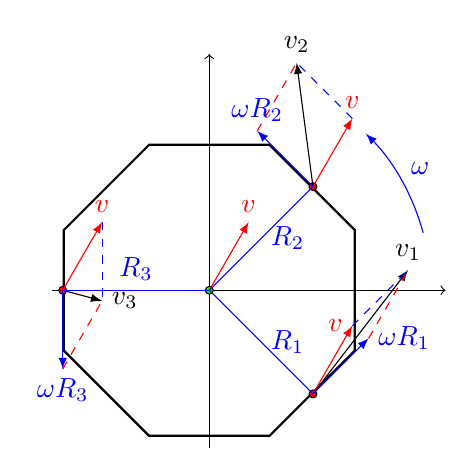
\begin{tikzpicture}
                    \draw [->] (-2, 0) -- (3, 0);
                    \draw [->] (0, -2) -- (0, 3);
                    \coordinate (o) at (0, 0);
                    \coordinate (v) at (0.5, {sqrt(3) / 2});
                    \coordinate (x) at ({+sqrt(2) / 2}, {sqrt(2) / 2});
                    \coordinate (y) at ({-sqrt(2) / 2}, {sqrt(2) / 2});
                    \coordinate (z) at (0, -1);
                    \draw (o) node [draw, thick, minimum size=4cm, name=O, regular polygon, regular polygon sides=8] {};
                    \draw (O) node [fill=green, circle, draw, inner sep=1pt] {};
                    \coordinate (a) at (O.side 6);
                    \coordinate (b) at (O.side 8);
                    \coordinate (c) at (O.side 3);
                    \coordinate (d) at (O.side 7);
                    \coordinate (e) at ($ (d) + (0, 0.5) $);
                    \coordinate (f) at ($ (a) + (1, 0) $);
                    \coordinate (g) at ($ (b) + (1, 0) $);
                    \coordinate (h) at ($ (c) + (1, 0) $);
                    \coordinate (i) at ($ (a) + (v) + (x) $);
                    \coordinate (j) at ($ (b) + (v) + (y) $);
                    \coordinate (k) at ($ (c) + (v) + (z) $);
                    \draw (a) node [fill=red, circle, draw, inner sep=1pt] {};
                    \draw (b) node [fill=red, circle, draw, inner sep=1pt] {};
                    \draw (c) node [fill=red, circle, draw, inner sep=1pt] {};
                    \draw [->, -latex, red] (o) -- (v) node [above] {$v$};
                    \pic [blue, draw, ->, -latex, "$\omega$", angle eccentricity=1.1, angle radius=80] {angle = e--o--b};
                    \draw [->, -latex] (a) -- (i) node [above] {$v_1$};
                    \draw [->, -latex] (b) -- (j) node [above] {$v_2$};
                    \draw [->, -latex] (c) -- (k) node [right] {$v_3$};

                    \draw [blue] (o) -- (a) node [pos=0.5, right] {$R_1$};
                    \draw [blue] (o) -- (b) node [pos=0.5, right] {$R_2$};
                    \draw [blue] (o) -- (c) node [pos=0.5, above] {$R_3$};
                    \draw [->, -latex, red] (a) -- ++(v) node [left] {$v$};
                    \draw [->, -latex, red] (b) -- ++(v) node [above] {$v$};
                    \draw [->, -latex, red] (c) -- ++(v) node [above] {$v$};
                    \draw [->, -latex, blue] (a) -- ++(x) node [right] {$\omega R_1$};
                    \draw [->, -latex, blue] (b) -- ++(y) node [above] {$\omega R_2$};
                    \draw [->, -latex, blue] (c) -- ++(z) node [below] {$\omega R_3$};
                    \draw [blue, dashed] ($ (a) + (v) $) -- (i);
                    \draw [blue, dashed] ($ (b) + (v) $) -- (j);
                    \draw [blue, dashed] ($ (c) + (v) $) -- (k);
                    \draw [red, dashed] ($ (a) + (x) $) -- (i);
                    \draw [red, dashed] ($ (b) + (y) $) -- (j);
                    \draw [red, dashed] ($ (c) + (z) $) -- (k);
                \end{tikzpicture}
                \caption{Geometrical construction of $(v_i, \theta_i)$}
            \end{subfigure}

            \caption{$(v_i, \theta_i)$ as a function of $(v, \theta, \omega)$}
            \label{octogon}
        \end{figure}

        \begin{itemize}
            \item Présentation générale (schéma octogone avec le CIR)
            \item Schéma bloc
            \item captures d’écran du simulateur
        \end{itemize}


        \section{Implementation}

        Photos

        \begin{itemize}
            \item sondes granier
            \item AGV désossé
            \item photo de pose des balises dans l’arbre
            \item arbre en acheminement
        \end{itemize}


        déroulement du projet
        jusqu’à l’inauguration de la ministre

        \section{Conclusion}


        \section*{APPENDIX}
        \section*{ACKNOWLEDGMENT}
        \addtolength{\textheight}{-12cm}  % TODO
        \end{document}
